\RequirePackage[l2tabu, orthodox]{nag}
\documentclass[12pt]{article}
\usepackage[T1]{fontenc}
\usepackage[utf8]{inputenc}
\usepackage[french]{babel}
\usepackage{amsthm,amssymb,amsmath,xcolor}
\usepackage{setspace}
\doublespacing
\usepackage{geometry}
\geometry{
    a4paper,
    total={170mm,257mm},
}
\usepackage{graphicx}
\graphicspath{ {./} }
\usepackage{microtype}
\usepackage{todonotes}
\usepackage{hyperref}
\hypersetup{
    colorlinks=true,
    linkcolor=blue,
    filecolor=magenta,
    urlcolor=cyan,
}

\author{Efe ERKEN}
\date{\today}
\title{Rapport Projet ``Liste de tâches''}

\begin{document}
\maketitle

\section{Modèle E/A}
\begin{center}
	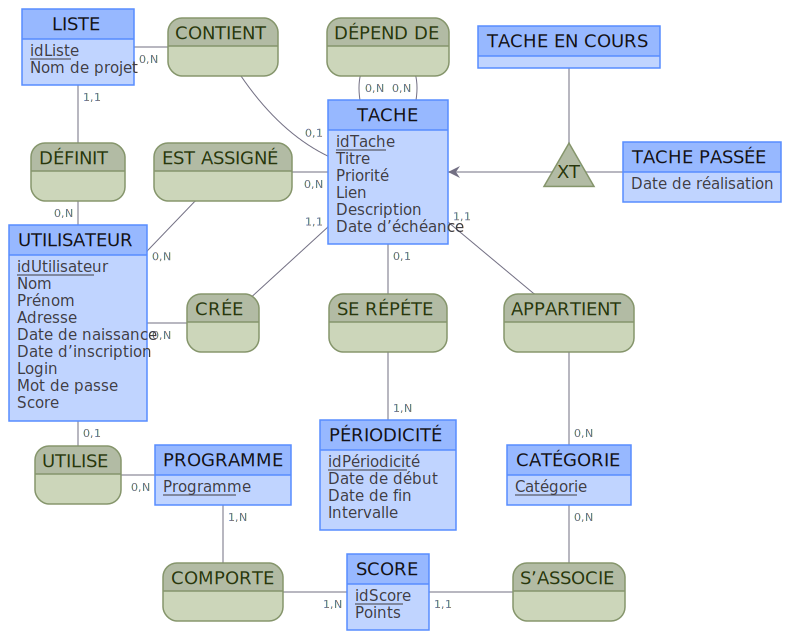
\includegraphics[scale=0.8]{modeleEA.png}
\end{center}

\section{Modèle relationnel}
\input{mld.tex}

\section{Choix d'implémentation}
Tout d'abord, petit avertissement. J'ai fait le choix d'utiliser
\href{https://dbeaver.io/}{\texttt{DBeaver}} comme client SQL et environnement
de dévéloppement. J'ai testé et assuré fonctionnel mon travail à l'aide de cet
outil. C'est pour cette raison que des erreurs peuvent se manifester à
l'execution avec d'autres outils comme \texttt{SQLplus} ou \texttt{SQL
	Developer}. Je n'ai pas conduit de tests avec ces outils mais je sais que
certaines formes de syntaxe \texttt{DBeaver} ne marche pas sur \texttt{SQLplus}
et vice-versa. (Notamment il ne se trouve pas le charactère ``\texttt{/}'' dans
mes scripts qui est nécessaire avec \texttt{SQLplus}.) \\

Ensuite, j'ai respecté les détails du sujet dans la limite de ma compréhension
de ce dernier. Dans mon implémentation, il y a bien deux tables pour les tâches
actuelles et les tâches passées. De ce fait, certaines contraintes d'intégrité
comme la clé primaire qui sont d'habitude statiques, ne seront assuré que
dynamiquement. C'est à dire, à l'aide des déclencheurs sur les deux tables
tâche, les tables qui réfèrent aux tâches ainsi que sur la vue qui regroupe
toutes les tâches en un endroit pour s'assurer que sur l'ensemble des deux
tables tâche, les identifiants soient unique et que les tables qui ont comme
clé étrangère des tâches, réfèrent bien à des tâches existantes. Ces
déclencheurs vont aussi servir à effacer en cascade les n-uplets qui réfèrent à
des tâches qui viennent d'être supprimées. Tous ceux qui réfèrent à des tâches
vont devoir avoir des déclancheur pour assurer l'intégrité. D'autres
contraintes qui nécessitent de lire des tables ou des comparaisons avec la date
actuelle vont aussi devoir être implémentées dynamiquement. \\

Une liste et un projet sont vus comme la même entité. Au lieu d'avoir une autre
table projet, j'ai integré un attribut ``nom de projet'' dans la table liste.
Une liste est un projet, un projet est une liste. C'est une manière d'organiser
ses tâches tout simplement. \\

Les listes vides (avec aucune tâche comme contenu) sont autorisées. Les tâches
peuvent être dans aucune liste. Toute tâche appartient à un utilisateur qui est
son créateur logiquement parlant, cela est stocké en tant qu'attribut dans une
tâche. Les utilisateurs ne peuvent pas être assignés à leurs propres tâches.
Une tâche ne peut pas dépendre d'elle même, non plus d'intérdependence entre
des tâches (cycles). \\

Le score est stocké en tant qu'attribut dans la table utilisateur. Le programme
est un type composé qui s'agit d'un couple de nombres, le premier indiquant le
nombre de points à ajouter et le deuxième le nombre de points à retirer. Il est
aussi un attribut de la table utilisateur. Je pense ne pas avoir bien compris
l'idée derrière ce concept de ``programme'' propre à chaque utilisateur, chaque
utilisateur étant libre d'en spécifier un ou pas. En plus il y a un système de
niveau mais le calcul pour lequel est statique d'après le sujet. C'est à dire
un calcul de score qui s'adapte pas au grandeur des points dans un programme
spécifé. Les utilisateurs peuvent donc renseigner un programme qui leur fait
gagner plein de points et qui retire jamais de points pour sauter de niveaux
plus facilement et tricher. Cela rend l'idée d'avoir un système de score
inutile et sans de vrai valeur. Mais tout de même, j'ai essayé de faire comme
je l'ai compris. Peut-être que ce n'est pas censé être une fonctionnalité
sociale mais privée pour que chaque utilisateur puisse suivre son évolution au
fil du temps de son coté.

\input{contraintes.tex}


\end{document}

